\documentclass[
  man,
  floatsintext,
  longtable,
  nolmodern,
  notxfonts,
  notimes,
  colorlinks=true,linkcolor=blue,citecolor=blue,urlcolor=blue]{apa7}

\usepackage{amsmath}
\usepackage{amssymb}



\usepackage[bidi=default]{babel}
\babelprovide[main,import]{american}


% get rid of language-specific shorthands (see #6817):
\let\LanguageShortHands\languageshorthands
\def\languageshorthands#1{}

\RequirePackage{longtable}
\RequirePackage{threeparttablex}

\makeatletter
\renewcommand{\paragraph}{\@startsection{paragraph}{4}{\parindent}%
	{0\baselineskip \@plus 0.2ex \@minus 0.2ex}%
	{-.5em}%
	{\normalfont\normalsize\bfseries\typesectitle}}

\renewcommand{\subparagraph}[1]{\@startsection{subparagraph}{5}{0.5em}%
	{0\baselineskip \@plus 0.2ex \@minus 0.2ex}%
	{-\z@\relax}%
	{\normalfont\normalsize\bfseries\itshape\hspace{\parindent}{#1}\textit{\addperi}}{\relax}}
\makeatother




\usepackage{longtable, booktabs, multirow, multicol, colortbl, hhline, caption, array, float, xpatch}
\usepackage{subcaption}
\renewcommand\thesubfigure{\Alph{subfigure}}
\setcounter{topnumber}{2}
\setcounter{bottomnumber}{2}
\setcounter{totalnumber}{4}
\renewcommand{\topfraction}{0.85}
\renewcommand{\bottomfraction}{0.85}
\renewcommand{\textfraction}{0.15}
\renewcommand{\floatpagefraction}{0.7}

\usepackage{tcolorbox}
\tcbuselibrary{listings,theorems, breakable, skins}
\usepackage{fontawesome5}

\definecolor{quarto-callout-color}{HTML}{909090}
\definecolor{quarto-callout-note-color}{HTML}{0758E5}
\definecolor{quarto-callout-important-color}{HTML}{CC1914}
\definecolor{quarto-callout-warning-color}{HTML}{EB9113}
\definecolor{quarto-callout-tip-color}{HTML}{00A047}
\definecolor{quarto-callout-caution-color}{HTML}{FC5300}
\definecolor{quarto-callout-color-frame}{HTML}{ACACAC}
\definecolor{quarto-callout-note-color-frame}{HTML}{4582EC}
\definecolor{quarto-callout-important-color-frame}{HTML}{D9534F}
\definecolor{quarto-callout-warning-color-frame}{HTML}{F0AD4E}
\definecolor{quarto-callout-tip-color-frame}{HTML}{02B875}
\definecolor{quarto-callout-caution-color-frame}{HTML}{FD7E14}

%\newlength\Oldarrayrulewidth
%\newlength\Oldtabcolsep


\usepackage{hyperref}



\usepackage{color}
\usepackage{fancyvrb}
\newcommand{\VerbBar}{|}
\newcommand{\VERB}{\Verb[commandchars=\\\{\}]}
\DefineVerbatimEnvironment{Highlighting}{Verbatim}{commandchars=\\\{\}}
% Add ',fontsize=\small' for more characters per line
\usepackage{framed}
\definecolor{shadecolor}{RGB}{241,243,245}
\newenvironment{Shaded}{\begin{snugshade}}{\end{snugshade}}
\newcommand{\AlertTok}[1]{\textcolor[rgb]{0.68,0.00,0.00}{#1}}
\newcommand{\AnnotationTok}[1]{\textcolor[rgb]{0.37,0.37,0.37}{#1}}
\newcommand{\AttributeTok}[1]{\textcolor[rgb]{0.40,0.45,0.13}{#1}}
\newcommand{\BaseNTok}[1]{\textcolor[rgb]{0.68,0.00,0.00}{#1}}
\newcommand{\BuiltInTok}[1]{\textcolor[rgb]{0.00,0.23,0.31}{#1}}
\newcommand{\CharTok}[1]{\textcolor[rgb]{0.13,0.47,0.30}{#1}}
\newcommand{\CommentTok}[1]{\textcolor[rgb]{0.37,0.37,0.37}{#1}}
\newcommand{\CommentVarTok}[1]{\textcolor[rgb]{0.37,0.37,0.37}{\textit{#1}}}
\newcommand{\ConstantTok}[1]{\textcolor[rgb]{0.56,0.35,0.01}{#1}}
\newcommand{\ControlFlowTok}[1]{\textcolor[rgb]{0.00,0.23,0.31}{\textbf{#1}}}
\newcommand{\DataTypeTok}[1]{\textcolor[rgb]{0.68,0.00,0.00}{#1}}
\newcommand{\DecValTok}[1]{\textcolor[rgb]{0.68,0.00,0.00}{#1}}
\newcommand{\DocumentationTok}[1]{\textcolor[rgb]{0.37,0.37,0.37}{\textit{#1}}}
\newcommand{\ErrorTok}[1]{\textcolor[rgb]{0.68,0.00,0.00}{#1}}
\newcommand{\ExtensionTok}[1]{\textcolor[rgb]{0.00,0.23,0.31}{#1}}
\newcommand{\FloatTok}[1]{\textcolor[rgb]{0.68,0.00,0.00}{#1}}
\newcommand{\FunctionTok}[1]{\textcolor[rgb]{0.28,0.35,0.67}{#1}}
\newcommand{\ImportTok}[1]{\textcolor[rgb]{0.00,0.46,0.62}{#1}}
\newcommand{\InformationTok}[1]{\textcolor[rgb]{0.37,0.37,0.37}{#1}}
\newcommand{\KeywordTok}[1]{\textcolor[rgb]{0.00,0.23,0.31}{\textbf{#1}}}
\newcommand{\NormalTok}[1]{\textcolor[rgb]{0.00,0.23,0.31}{#1}}
\newcommand{\OperatorTok}[1]{\textcolor[rgb]{0.37,0.37,0.37}{#1}}
\newcommand{\OtherTok}[1]{\textcolor[rgb]{0.00,0.23,0.31}{#1}}
\newcommand{\PreprocessorTok}[1]{\textcolor[rgb]{0.68,0.00,0.00}{#1}}
\newcommand{\RegionMarkerTok}[1]{\textcolor[rgb]{0.00,0.23,0.31}{#1}}
\newcommand{\SpecialCharTok}[1]{\textcolor[rgb]{0.37,0.37,0.37}{#1}}
\newcommand{\SpecialStringTok}[1]{\textcolor[rgb]{0.13,0.47,0.30}{#1}}
\newcommand{\StringTok}[1]{\textcolor[rgb]{0.13,0.47,0.30}{#1}}
\newcommand{\VariableTok}[1]{\textcolor[rgb]{0.07,0.07,0.07}{#1}}
\newcommand{\VerbatimStringTok}[1]{\textcolor[rgb]{0.13,0.47,0.30}{#1}}
\newcommand{\WarningTok}[1]{\textcolor[rgb]{0.37,0.37,0.37}{\textit{#1}}}

\providecommand{\tightlist}{%
  \setlength{\itemsep}{0pt}\setlength{\parskip}{0pt}}
\usepackage{longtable,booktabs,array}
\usepackage{calc} % for calculating minipage widths
% Correct order of tables after \paragraph or \subparagraph
\usepackage{etoolbox}
\makeatletter
\patchcmd\longtable{\par}{\if@noskipsec\mbox{}\fi\par}{}{}
\makeatother
% Allow footnotes in longtable head/foot
\IfFileExists{footnotehyper.sty}{\usepackage{footnotehyper}}{\usepackage{footnote}}
\makesavenoteenv{longtable}

\usepackage{graphicx}
\makeatletter
\newsavebox\pandoc@box
\newcommand*\pandocbounded[1]{% scales image to fit in text height/width
  \sbox\pandoc@box{#1}%
  \Gscale@div\@tempa{\textheight}{\dimexpr\ht\pandoc@box+\dp\pandoc@box\relax}%
  \Gscale@div\@tempb{\linewidth}{\wd\pandoc@box}%
  \ifdim\@tempb\p@<\@tempa\p@\let\@tempa\@tempb\fi% select the smaller of both
  \ifdim\@tempa\p@<\p@\scalebox{\@tempa}{\usebox\pandoc@box}%
  \else\usebox{\pandoc@box}%
  \fi%
}
% Set default figure placement to htbp
\def\fps@figure{htbp}
\makeatother


% definitions for citeproc citations
\NewDocumentCommand\citeproctext{}{}
\NewDocumentCommand\citeproc{mm}{%
  \begingroup\def\citeproctext{#2}\cite{#1}\endgroup}
\makeatletter
 % allow citations to break across lines
 \let\@cite@ofmt\@firstofone
 % avoid brackets around text for \cite:
 \def\@biblabel#1{}
 \def\@cite#1#2{{#1\if@tempswa , #2\fi}}
\makeatother
\newlength{\cslhangindent}
\setlength{\cslhangindent}{1.5em}
\newlength{\csllabelwidth}
\setlength{\csllabelwidth}{3em}
\newenvironment{CSLReferences}[2] % #1 hanging-indent, #2 entry-spacing
 {\begin{list}{}{%
  \setlength{\itemindent}{0pt}
  \setlength{\leftmargin}{0pt}
  \setlength{\parsep}{0pt}
  % turn on hanging indent if param 1 is 1
  \ifodd #1
   \setlength{\leftmargin}{\cslhangindent}
   \setlength{\itemindent}{-1\cslhangindent}
  \fi
  % set entry spacing
  \setlength{\itemsep}{#2\baselineskip}}}
 {\end{list}}
\usepackage{calc}
\newcommand{\CSLBlock}[1]{\hfill\break\parbox[t]{\linewidth}{\strut\ignorespaces#1\strut}}
\newcommand{\CSLLeftMargin}[1]{\parbox[t]{\csllabelwidth}{\strut#1\strut}}
\newcommand{\CSLRightInline}[1]{\parbox[t]{\linewidth - \csllabelwidth}{\strut#1\strut}}
\newcommand{\CSLIndent}[1]{\hspace{\cslhangindent}#1}





\usepackage{newtx}

\defaultfontfeatures{Scale=MatchLowercase}
\defaultfontfeatures[\rmfamily]{Ligatures=TeX,Scale=1}





\title{The Importance of Summary Statistics and Techniques for Creating
Them in R}


\shorttitle{Summary Statistics and Techniques in R}


\usepackage{etoolbox}






\author{Jelin George (Matriculation: 400826617)}



\affiliation{
{Hochschule Fresenius - University of Applied Science}}




\leftheader{400826617)}



\abstract{This document presents a concise overview of summary
statistics and their importance in R. Summary statistics - such as mean,
median, standard deviation, and frequency counts - capture the key
features of a dataset, enabling quick exploration and interpretation. R
provides powerful functions and visualization tools to efficiently
compute and present these statistics, making them essential for
simplifying data, identifying patterns, and supporting informed analysis
and decision-making. Practical examples and code are provided to
demonstrate these concepts in action. The document also discusses the
limitations of summary statistics and considers future directions in
their application. }

\keywords{summary statistics, R programming, data analysis, descriptive
statistics, data visualization, exploratory data analysis, limitations}

\authornote{ 
\par{ }
\par{   The authors have no conflicts of interest to disclose.    }
\par{Correspondence concerning this article should be addressed to Jelin
George (Matriculation:
400826617), Email: \href{mailto:george.jelin@stud-hs.fresenius.de}{george.jelin@stud-hs.fresenius.de}}
}

\makeatletter
\let\endoldlt\endlongtable
\def\endlongtable{
\hline
\endoldlt
}
\makeatother

\urlstyle{same}



\usepackage{booktabs}
\usepackage{longtable}
\usepackage{array}
\usepackage{multirow}
\usepackage{wrapfig}
\usepackage{float}
\usepackage{colortbl}
\usepackage{pdflscape}
\usepackage{tabu}
\usepackage{threeparttable}
\usepackage{threeparttablex}
\usepackage[normalem]{ulem}
\usepackage{makecell}
\usepackage{xcolor}
\makeatletter
\@ifpackageloaded{caption}{}{\usepackage{caption}}
\AtBeginDocument{%
\ifdefined\contentsname
  \renewcommand*\contentsname{Table of contents}
\else
  \newcommand\contentsname{Table of contents}
\fi
\ifdefined\listfigurename
  \renewcommand*\listfigurename{List of Figures}
\else
  \newcommand\listfigurename{List of Figures}
\fi
\ifdefined\listtablename
  \renewcommand*\listtablename{List of Tables}
\else
  \newcommand\listtablename{List of Tables}
\fi
\ifdefined\figurename
  \renewcommand*\figurename{Figure}
\else
  \newcommand\figurename{Figure}
\fi
\ifdefined\tablename
  \renewcommand*\tablename{Table}
\else
  \newcommand\tablename{Table}
\fi
}
\@ifpackageloaded{float}{}{\usepackage{float}}
\floatstyle{ruled}
\@ifundefined{c@chapter}{\newfloat{codelisting}{h}{lop}}{\newfloat{codelisting}{h}{lop}[chapter]}
\floatname{codelisting}{Listing}
\newcommand*\listoflistings{\listof{codelisting}{List of Listings}}
\makeatother
\makeatletter
\makeatother
\makeatletter
\@ifpackageloaded{caption}{}{\usepackage{caption}}
\@ifpackageloaded{subcaption}{}{\usepackage{subcaption}}
\makeatother

% From https://tex.stackexchange.com/a/645996/211326
%%% apa7 doesn't want to add appendix section titles in the toc
%%% let's make it do it
\makeatletter
\xpatchcmd{\appendix}
  {\par}
  {\addcontentsline{toc}{section}{\@currentlabelname}\par}
  {}{}
\makeatother

%% Disable longtable counter
%% https://tex.stackexchange.com/a/248395/211326

\usepackage{etoolbox}

\makeatletter
\patchcmd{\LT@caption}
  {\bgroup}
  {\bgroup\global\LTpatch@captiontrue}
  {}{}
\patchcmd{\longtable}
  {\par}
  {\par\global\LTpatch@captionfalse}
  {}{}
\apptocmd{\endlongtable}
  {\ifLTpatch@caption\else\addtocounter{table}{-1}\fi}
  {}{}
\newif\ifLTpatch@caption
\makeatother

\begin{document}

\maketitle

\hypertarget{toc}{}
\tableofcontents
\newpage
\section[Introduction]{The Importance of Summary Statistics and
Techniques for Creating Them in R}

\setcounter{secnumdepth}{-\maxdimen} % remove section numbering

\setlength\LTleft{0pt}


Summary statistics are numerical values that describe the main features
of a dataset, such as its center and spread. They simplify complex data
into easily interpretable numbers, offering quick insights into trends
and variability, and serve as a foundation for further analysis. These
statistics provide a snapshot of the data, facilitating initial
exploration, quality checks, and communication of results. In R, these
statistics not only reveal patterns and outliers but also lay the
groundwork for informed decision-making.

In this document, we will:

\begin{itemize}
\item
  Define summary statistics and their importance
\item
  Explore key measures and techniques
\item
  Demonstrate practical application with code
\item
  Analyze limitations and consider furture directions
\end{itemize}

\newpage

\section{What is Summary Statistics?}\label{what-is-summary-statistics}

Summary statistics are concise numerical measures that capture the
essential characteristics of a dataset. They serve as foundational tools
in data analysis, providing concise descriptions of large datasets. They
help analysts and researchers understand the central tendencies,
variability, and overall distribution of data, making complex datasets
interpretable and actionable. Without summary statistics, raw data would
be overwhelming and difficult to interpret, making it challenging to
draw meaningful conclusions or communicate findings effectively.

In R, summary statistics are foundational for data analysis, enabling
users to efficiently condense complex data into interpretable values
like the mean, median, mode, standard deviation, and quantiles. R offers
a rich ecosystem of functions and packages - such as summary(),
dplyr::summarise(), and visualization tools like histograms and boxplots
- that streamline the computation and presentation of summary statistics
for both numeric and categorical data. Their importance lies in
simplifying large datasets, revealing patterns and outliers, and laying
the groundwork for deeper statistical analyses and informed
decision-making.

As the first and often most critical step in any analytical workflow,
summary statistics in R empower analysts and researchers to understand,
compare, and communicate data-driven insights with clarity and
precision.

Summary statistics can be typically divided into:

\begin{enumerate}
\def\labelenumi{\arabic{enumi}.}
\item
  \textbf{Descriptive statistics}: Summarize the main features of a
  dataset (e.g., mean, median, mode). \emph{This will be our focus
  here.}
\item
  \textbf{Inferential statistics}: Make predictions or inferences about
  a population based on a sample.
\end{enumerate}

I would like to highlight a book, \emph{Making sense of statistics: A
conceptual overview}, (\citeproc{ref-oh2023making}{Oh \& Pyrczak, 2023})
which offers a clear and accessible introduction to key statistical
concepts for beginners. The book focuses on building conceptual
understanding of both descriptive and inferential statistics, using
simple explanations, practical examples, and step-by-step guidance. It
is designed to help in applying statistics to research and interpreting
data effectively.

Additonally, watch this
\href{https://www.youtube.com/watch?v=yoPGwvUzjgQ}{\textbf{tutorial
video}} on descriptive statistics in R to get you started.

\begin{longtable}[]{@{}
  >{\raggedright\arraybackslash}p{(\linewidth - 6\tabcolsep) * \real{0.0977}}
  >{\raggedright\arraybackslash}p{(\linewidth - 6\tabcolsep) * \real{0.1955}}
  >{\raggedright\arraybackslash}p{(\linewidth - 6\tabcolsep) * \real{0.4060}}
  >{\raggedright\arraybackslash}p{(\linewidth - 6\tabcolsep) * \real{0.3008}}@{}}
\caption{Comparison of R Summary Packages}\tabularnewline
\toprule\noalign{}
\begin{minipage}[b]{\linewidth}\raggedright
Package
\end{minipage} & \begin{minipage}[b]{\linewidth}\raggedright
Key\_Functions
\end{minipage} & \begin{minipage}[b]{\linewidth}\raggedright
Strengths
\end{minipage} & \begin{minipage}[b]{\linewidth}\raggedright
Use\_Case
\end{minipage} \\
\midrule\noalign{}
\endfirsthead
\toprule\noalign{}
\begin{minipage}[b]{\linewidth}\raggedright
Package
\end{minipage} & \begin{minipage}[b]{\linewidth}\raggedright
Key\_Functions
\end{minipage} & \begin{minipage}[b]{\linewidth}\raggedright
Strengths
\end{minipage} & \begin{minipage}[b]{\linewidth}\raggedright
Use\_Case
\end{minipage} \\
\midrule\noalign{}
\endhead
\bottomrule\noalign{}
\endlastfoot
Base R & summary(), mean(), sd() & Built-in, quick, basic, not pipeable
& General, quick checks \\
dplyr & summarise(), count() & Tidy, pipeable, flexible, group-wise
summaries & Custom summaries in tidyverse workflows \\
skimr & skim() & Tidy, detailed, sparkline histograms, missing data &
Quick, detailed EDA \\
psych & describe(), describe.by() & Skewness, kurtosis, group summaries
& In-depth descriptive stats \\
summarytools & descr(), dfSummary() & HTML summaries, mini-histograms,
missing data info & Publication-ready summaries \\
Hmisc & describe() & Detailed, percentiles, unique values & Medical,
epidemiological data \\
pastecs & stat.desc() & Wide range of stats, time series support &
Broad, one-call summaries \\
mosaic & favstats(), tally() & Concise, teaching-focused & Teaching,
quick summaries \\
gtsummary & tbl\_summary() & Publication-ready tables, auto-detects
variable types & Medical, scientific reporting \\
\end{longtable}

\newpage

\section{Key Measures in Summary
Statistics}\label{key-measures-in-summary-statistics}

Summary statistics condense complex datasets into a few meaningful
numbers, making it easier to understand and communicate data
characteristics. The key measures in summary statistics fall into
several categories:

\subsection{Measures of Central
Tendency}\label{measures-of-central-tendency}

Central tendency measures indicate where most values in a dataset fall.

\begin{itemize}
\item
  \textbf{Mean}: The arithmetic average of all data points. Add up all
  the values, then divide by how many there are to get the average of
  all the numbers.
\item
  \textbf{Median}: The middle value when data is ordered. If there's an
  even number, it's the average of the two middle numbers.
\item
  \textbf{Mode}: The most frequently occurring value.
\end{itemize}

\begin{Shaded}
\begin{Highlighting}[]
\CommentTok{\# Example in R}

\CommentTok{\#| echo: true}
\CommentTok{\#| label: mean{-}median{-}mode}
\NormalTok{data\_tbl }\OtherTok{\textless{}{-}} \FunctionTok{tibble}\NormalTok{(}\AttributeTok{value =} \FunctionTok{c}\NormalTok{(}\DecValTok{2}\NormalTok{, }\DecValTok{4}\NormalTok{, }\DecValTok{4}\NormalTok{, }\DecValTok{4}\NormalTok{, }\DecValTok{5}\NormalTok{, }\DecValTok{7}\NormalTok{, }\DecValTok{9}\NormalTok{))}

\NormalTok{data\_tbl }\SpecialCharTok{\%\textgreater{}\%}
  \FunctionTok{summarise}\NormalTok{(}
    \AttributeTok{mean =} \FunctionTok{mean}\NormalTok{(value),}
    \AttributeTok{median =} \FunctionTok{median}\NormalTok{(value),}
    \AttributeTok{mode =}\NormalTok{ value }\SpecialCharTok{\%\textgreater{}\%} 
      \FunctionTok{table}\NormalTok{() }\SpecialCharTok{\%\textgreater{}\%} 
      \FunctionTok{which.max}\NormalTok{() }\SpecialCharTok{\%\textgreater{}\%} 
      \FunctionTok{names}\NormalTok{() }\SpecialCharTok{\%\textgreater{}\%} 
      \FunctionTok{as.numeric}\NormalTok{()}
\NormalTok{  )}
\end{Highlighting}
\end{Shaded}

\begin{verbatim}
# A tibble: 1 x 3
   mean median  mode
  <dbl>  <dbl> <dbl>
1     5      4     4
\end{verbatim}

\subsection{Measures of Dispersion}\label{measures-of-dispersion}

Dispersion measures describe the spread of data.

\begin{figure}[!htbp]

{\caption{{Distributions With Different
Dispersion}{\label{fig-dispersion}}}}

\pandocbounded{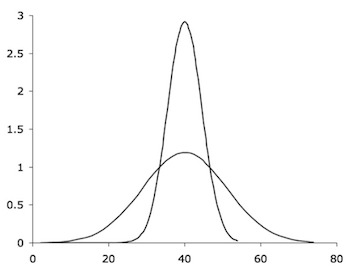
\includegraphics[keepaspectratio]{Dispersionimage.png}}

{\noindent \emph{Note.} Example of samples from two populations with the
same mean but different dispersion. The blue population is much more
dispersed than the red population.}

\end{figure}

\emph{Source: https://en.wikipedia.org/wiki/Statistical\_dispersion}

\begin{itemize}
\item
  \textbf{Range}: Difference between max and min values.
\item
  \textbf{Variance}: Average squared deviation from the mean.
\item
  \textbf{Standard Deviation}: Square root of variance.
\item
  \textbf{Interquartile Range (IQR)}: Range between the 25th and 75th
  percentiles.
\item
  \textbf{Coefficient of Variation}: Standard deviation divided by the
  mean.
\end{itemize}

\begin{Shaded}
\begin{Highlighting}[]
\NormalTok{data\_tbl }\OtherTok{\textless{}{-}} \FunctionTok{tibble}\NormalTok{(}\AttributeTok{value =} \FunctionTok{c}\NormalTok{(}\DecValTok{2}\NormalTok{, }\DecValTok{4}\NormalTok{, }\DecValTok{4}\NormalTok{, }\DecValTok{4}\NormalTok{, }\DecValTok{5}\NormalTok{, }\DecValTok{7}\NormalTok{, }\DecValTok{9}\NormalTok{))}

\NormalTok{data\_tbl }\SpecialCharTok{\%\textgreater{}\%}
  \FunctionTok{summarise}\NormalTok{(}
    \AttributeTok{min =} \FunctionTok{min}\NormalTok{(value),}
    \AttributeTok{max =} \FunctionTok{max}\NormalTok{(value),}
    \AttributeTok{range =} \FunctionTok{max}\NormalTok{(value) }\SpecialCharTok{{-}} \FunctionTok{min}\NormalTok{(value),}
    \AttributeTok{variance =} \FunctionTok{var}\NormalTok{(value),}
    \AttributeTok{sd =} \FunctionTok{sd}\NormalTok{(value),}
    \AttributeTok{IQR =} \FunctionTok{IQR}\NormalTok{(value),}
    \AttributeTok{coefficient\_of\_variation =} \FunctionTok{sd}\NormalTok{(value) }\SpecialCharTok{/} \FunctionTok{mean}\NormalTok{(value)}
\NormalTok{  )}
\end{Highlighting}
\end{Shaded}

\begin{verbatim}
# A tibble: 1 x 7
    min   max range variance    sd   IQR coefficient_of_variation
  <dbl> <dbl> <dbl>    <dbl> <dbl> <dbl>                    <dbl>
1     2     9     7     5.33  2.31     2                    0.462
\end{verbatim}

\subsection{Measures of Shape and
Distribution}\label{measures-of-shape-and-distribution}

Describe the overall pattern and characteristics of how data values are
distributed within a dataset.

\begin{itemize}
\tightlist
\item
  \textbf{Skewness}: Measures asymmetry of the distribution.
\item
  \textbf{Kurtosis}: Measures ``tailedness'' or peakedness of the
  distribution.
\end{itemize}

\begin{Shaded}
\begin{Highlighting}[]
\FunctionTok{library}\NormalTok{(dplyr)}

\NormalTok{data\_tbl }\OtherTok{\textless{}{-}} \FunctionTok{tibble}\NormalTok{(}\AttributeTok{value =} \FunctionTok{c}\NormalTok{(}\DecValTok{2}\NormalTok{, }\DecValTok{4}\NormalTok{, }\DecValTok{4}\NormalTok{, }\DecValTok{4}\NormalTok{, }\DecValTok{5}\NormalTok{, }\DecValTok{7}\NormalTok{, }\DecValTok{9}\NormalTok{))}

\NormalTok{data\_tbl }\SpecialCharTok{\%\textgreater{}\%}
  \FunctionTok{summarise}\NormalTok{(}
    \AttributeTok{n =} \FunctionTok{n}\NormalTok{(),}
    \AttributeTok{mean =} \FunctionTok{mean}\NormalTok{(value),}
    \AttributeTok{sd =} \FunctionTok{sd}\NormalTok{(value),}
    \AttributeTok{skewness =} \FunctionTok{sum}\NormalTok{((value }\SpecialCharTok{{-}}\NormalTok{ mean) }\SpecialCharTok{\^{}} \DecValTok{3}\NormalTok{) }\SpecialCharTok{/}\NormalTok{ n }\SpecialCharTok{/}\NormalTok{ (sd }\SpecialCharTok{\^{}} \DecValTok{3}\NormalTok{),}
    \AttributeTok{kurtosis =} \FunctionTok{sum}\NormalTok{((value }\SpecialCharTok{{-}}\NormalTok{ mean) }\SpecialCharTok{\^{}} \DecValTok{4}\NormalTok{) }\SpecialCharTok{/}\NormalTok{ n }\SpecialCharTok{/}\NormalTok{ (sd }\SpecialCharTok{\^{}} \DecValTok{4}\NormalTok{)}
\NormalTok{  ) }\SpecialCharTok{\%\textgreater{}\%}
  \FunctionTok{select}\NormalTok{(}\SpecialCharTok{{-}}\NormalTok{mean, }\SpecialCharTok{{-}}\NormalTok{sd, }\SpecialCharTok{{-}}\NormalTok{n) }\CommentTok{\# remove intermediate columns if you only want skewness and kurtosis}
\end{Highlighting}
\end{Shaded}

\begin{verbatim}
# A tibble: 1 x 2
  skewness kurtosis
     <dbl>    <dbl>
1    0.487     1.79
\end{verbatim}

\textbf{Visualization tools to help understand distribution of data
better.}

\begin{itemize}
\tightlist
\item
  \textbf{Histogram}: It displays how data values are distributed across
  different intervals in patterns like bell-shaped (normal), J-shaped,
  or skewed distributions, as well as spot outliers and the overall
  spread of the data.
\end{itemize}

\begin{Shaded}
\begin{Highlighting}[]
\CommentTok{\# This histogram shows the distribution in the example we set previously.}

\FunctionTok{library}\NormalTok{(ggplot2)}
\FunctionTok{library}\NormalTok{(tibble)}

\CommentTok{\#| label: fig{-}histogram}
\CommentTok{\#| fig{-}cap: "Histogram of the data"}

\NormalTok{data\_tbl }\OtherTok{\textless{}{-}} \FunctionTok{tibble}\NormalTok{(}\AttributeTok{value =} \FunctionTok{c}\NormalTok{(}\DecValTok{2}\NormalTok{, }\DecValTok{4}\NormalTok{, }\DecValTok{4}\NormalTok{, }\DecValTok{4}\NormalTok{, }\DecValTok{5}\NormalTok{, }\DecValTok{7}\NormalTok{, }\DecValTok{9}\NormalTok{))}

\FunctionTok{ggplot}\NormalTok{(data\_tbl, }\FunctionTok{aes}\NormalTok{(}\AttributeTok{x =}\NormalTok{ value)) }\SpecialCharTok{+}
  \FunctionTok{geom\_histogram}\NormalTok{(}\AttributeTok{binwidth =} \DecValTok{1}\NormalTok{, }\AttributeTok{fill =} \StringTok{"blue"}\NormalTok{, }\AttributeTok{color =} \StringTok{"black"}\NormalTok{) }\SpecialCharTok{+}
  \FunctionTok{labs}\NormalTok{(}
    \AttributeTok{title =} \StringTok{"Figure 2. Histogram of Data"}\NormalTok{,}
    \AttributeTok{x =} \StringTok{"Value"}\NormalTok{,}
    \AttributeTok{y =} \StringTok{"Frequency"}
\NormalTok{  )}
\end{Highlighting}
\end{Shaded}

\pandocbounded{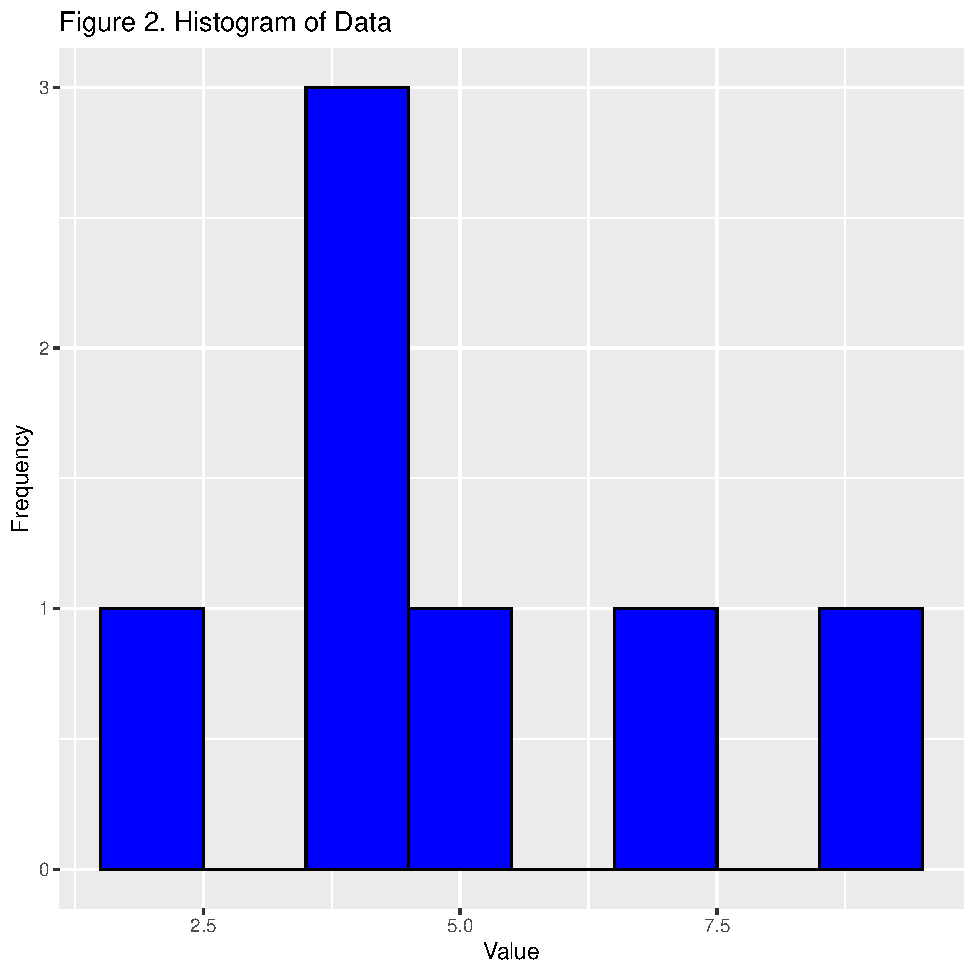
\includegraphics[keepaspectratio]{summarystatisticspdf_files/figure-pdf/unnamed-chunk-7-1.pdf}}

As seen above, the distribution is centered around 4.

\begin{itemize}
\tightlist
\item
  \textbf{Boxplot}: A graphical tool that visually summarizes the
  distribution, central tendency, spread, and skewness of numerical data
  using the five-number summary: minimum, first quartile (Q1), median,
  third quartile (Q3), and maximum.
\end{itemize}

\begin{Shaded}
\begin{Highlighting}[]
\FunctionTok{library}\NormalTok{(ggplot2)}
\FunctionTok{library}\NormalTok{(tibble)}

\NormalTok{data\_tbl }\OtherTok{\textless{}{-}} \FunctionTok{tibble}\NormalTok{(}\AttributeTok{value =} \FunctionTok{c}\NormalTok{(}\DecValTok{2}\NormalTok{, }\DecValTok{4}\NormalTok{, }\DecValTok{4}\NormalTok{, }\DecValTok{4}\NormalTok{, }\DecValTok{5}\NormalTok{, }\DecValTok{7}\NormalTok{, }\DecValTok{9}\NormalTok{))}

\FunctionTok{ggplot}\NormalTok{(data\_tbl, }\FunctionTok{aes}\NormalTok{(}\AttributeTok{x =} \FunctionTok{factor}\NormalTok{(}\DecValTok{1}\NormalTok{), }\AttributeTok{y =}\NormalTok{ value)) }\SpecialCharTok{+}
  \FunctionTok{geom\_boxplot}\NormalTok{(}\AttributeTok{fill =} \StringTok{"blue"}\NormalTok{) }\SpecialCharTok{+}
  \FunctionTok{labs}\NormalTok{(}
    \AttributeTok{title =} \StringTok{"Figure 3. Boxplot of Data"}\NormalTok{,}
    \AttributeTok{x =} \StringTok{""}\NormalTok{,}
    \AttributeTok{y =} \StringTok{"Value"}
\NormalTok{  ) }\SpecialCharTok{+}
  \FunctionTok{theme}\NormalTok{(}\AttributeTok{axis.text.x =} \FunctionTok{element\_blank}\NormalTok{(),}
        \AttributeTok{axis.ticks.x =} \FunctionTok{element\_blank}\NormalTok{())}
\end{Highlighting}
\end{Shaded}

\pandocbounded{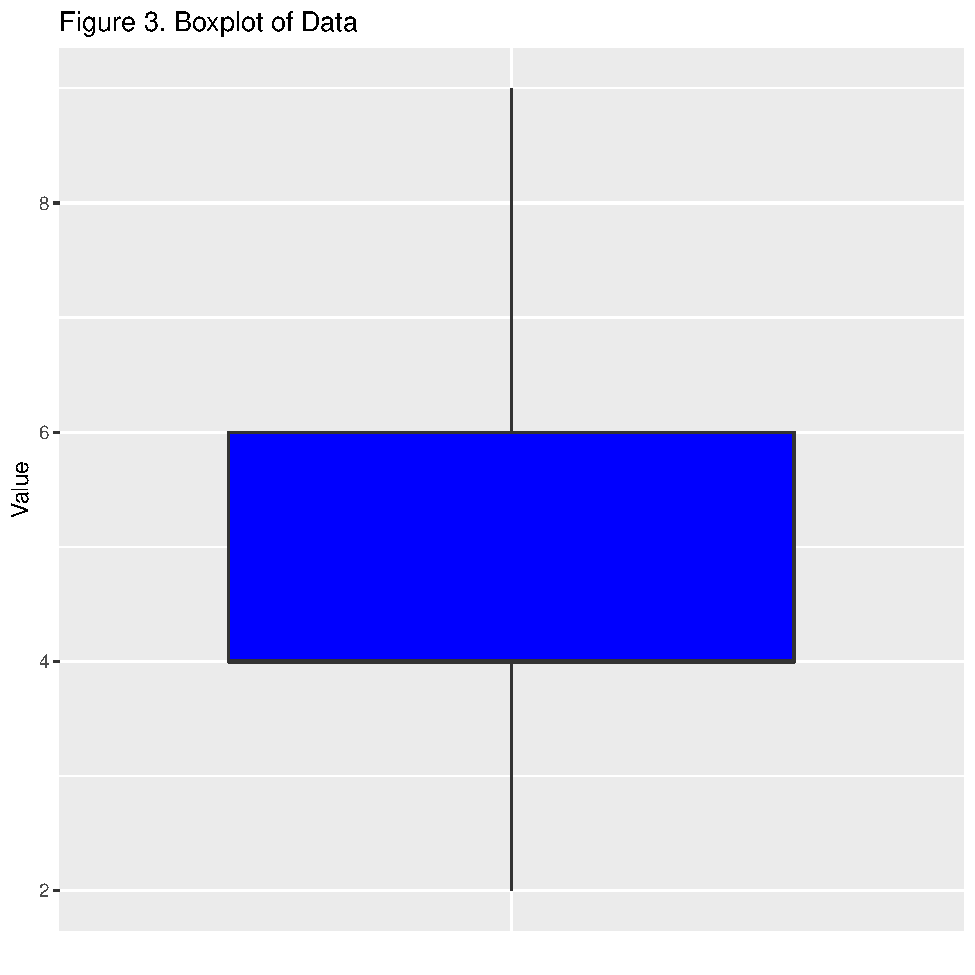
\includegraphics[keepaspectratio]{summarystatisticspdf_files/figure-pdf/unnamed-chunk-8-1.pdf}}

\subsection{Handling Missing Data}\label{handling-missing-data}

Missing data can bias summary statistics if not handled properly.

Types of missing data: MCAR (Missing Completely at Random), MAR (Missing
at Random), MNAR (Missing Not at Random).

Techniques: Omit missing values, impute with mean/median/mode, or use
advanced imputation.

\begin{Shaded}
\begin{Highlighting}[]
\NormalTok{data\_tbl }\OtherTok{\textless{}{-}} \FunctionTok{tibble}\NormalTok{(}\AttributeTok{value =} \FunctionTok{c}\NormalTok{(}\DecValTok{2}\NormalTok{, }\DecValTok{4}\NormalTok{, }\ConstantTok{NA}\NormalTok{, }\DecValTok{4}\NormalTok{, }\DecValTok{5}\NormalTok{, }\ConstantTok{NA}\NormalTok{, }\DecValTok{9}\NormalTok{))}

\NormalTok{data\_tbl }\SpecialCharTok{\%\textgreater{}\%}
  \FunctionTok{summarise}\NormalTok{(}\AttributeTok{mean =} \FunctionTok{mean}\NormalTok{(value, }\AttributeTok{na.rm =} \ConstantTok{TRUE}\NormalTok{)) }\CommentTok{\# Ignore NAs}
\end{Highlighting}
\end{Shaded}

\begin{verbatim}
# A tibble: 1 x 1
   mean
  <dbl>
1   4.8
\end{verbatim}

\subsection{Frequency and Cross-Tabulation
Techniques}\label{frequency-and-cross-tabulation-techniques}

\textbf{Frequency table}: A tool used to organize and display how often
each value or category occurs in a dataset. It typically consists of two
or more columns: one listing all possible values or categories, and
another showing the frequency (count) of each making it easier to see
which values are common or rare, summarize large sets of data, and
identify patterns.

\begin{itemize}
\tightlist
\item
  \textbf{Relative frequency}: Proportion of each category.
\item
  \textbf{Cumulative frequency}: Running total of frequencies.
\end{itemize}

\begin{Shaded}
\begin{Highlighting}[]
\CommentTok{\# Example data}
\NormalTok{age }\OtherTok{\textless{}{-}} \FunctionTok{c}\NormalTok{(}\StringTok{\textquotesingle{}Young\textquotesingle{}}\NormalTok{, }\StringTok{\textquotesingle{}Old\textquotesingle{}}\NormalTok{, }\StringTok{\textquotesingle{}Young\textquotesingle{}}\NormalTok{, }\StringTok{\textquotesingle{}Old\textquotesingle{}}\NormalTok{, }\StringTok{\textquotesingle{}Young\textquotesingle{}}\NormalTok{, }\StringTok{\textquotesingle{}Old\textquotesingle{}}\NormalTok{)}
\NormalTok{gender }\OtherTok{\textless{}{-}} \FunctionTok{c}\NormalTok{(}\StringTok{\textquotesingle{}Male\textquotesingle{}}\NormalTok{, }\StringTok{\textquotesingle{}Female\textquotesingle{}}\NormalTok{, }\StringTok{\textquotesingle{}Female\textquotesingle{}}\NormalTok{, }\StringTok{\textquotesingle{}Male\textquotesingle{}}\NormalTok{, }\StringTok{\textquotesingle{}Male\textquotesingle{}}\NormalTok{, }\StringTok{\textquotesingle{}Female\textquotesingle{}}\NormalTok{)}
\NormalTok{data\_tbl }\OtherTok{\textless{}{-}} \FunctionTok{tibble}\NormalTok{(}\AttributeTok{age =}\NormalTok{ age, }\AttributeTok{gender =}\NormalTok{ gender)}

\CommentTok{\# Frequency table for combinations of age and gender}
\NormalTok{data\_tbl }\SpecialCharTok{\%\textgreater{}\%}
  \FunctionTok{count}\NormalTok{(age, gender, }\AttributeTok{name =} \StringTok{"frequency"}\NormalTok{)}
\end{Highlighting}
\end{Shaded}

\begin{verbatim}
# A tibble: 4 x 3
  age   gender frequency
  <chr> <chr>      <int>
1 Old   Female         2
2 Old   Male           1
3 Young Female         1
4 Young Male           2
\end{verbatim}

\begin{Shaded}
\begin{Highlighting}[]
\CommentTok{\# Proportion table for combinations of age and gender}
\NormalTok{data\_tbl }\SpecialCharTok{\%\textgreater{}\%}
  \FunctionTok{count}\NormalTok{(age, gender, }\AttributeTok{name =} \StringTok{"frequency"}\NormalTok{) }\SpecialCharTok{\%\textgreater{}\%}
  \FunctionTok{mutate}\NormalTok{(}\AttributeTok{proportion =}\NormalTok{ frequency }\SpecialCharTok{/} \FunctionTok{sum}\NormalTok{(frequency))}
\end{Highlighting}
\end{Shaded}

\begin{verbatim}
# A tibble: 4 x 4
  age   gender frequency proportion
  <chr> <chr>      <int>      <dbl>
1 Old   Female         2      0.333
2 Old   Male           1      0.167
3 Young Female         1      0.167
4 Young Male           2      0.333
\end{verbatim}

\begin{Shaded}
\begin{Highlighting}[]
\CommentTok{\# To calculate the total of frequencies}
\NormalTok{age }\OtherTok{\textless{}{-}} \FunctionTok{c}\NormalTok{(}\StringTok{\textquotesingle{}Young\textquotesingle{}}\NormalTok{, }\StringTok{\textquotesingle{}Old\textquotesingle{}}\NormalTok{, }\StringTok{\textquotesingle{}Young\textquotesingle{}}\NormalTok{, }\StringTok{\textquotesingle{}Old\textquotesingle{}}\NormalTok{, }\StringTok{\textquotesingle{}Young\textquotesingle{}}\NormalTok{, }\StringTok{\textquotesingle{}Old\textquotesingle{}}\NormalTok{)}
\NormalTok{gender }\OtherTok{\textless{}{-}} \FunctionTok{c}\NormalTok{(}\StringTok{\textquotesingle{}Male\textquotesingle{}}\NormalTok{, }\StringTok{\textquotesingle{}Female\textquotesingle{}}\NormalTok{, }\StringTok{\textquotesingle{}Female\textquotesingle{}}\NormalTok{, }\StringTok{\textquotesingle{}Male\textquotesingle{}}\NormalTok{, }\StringTok{\textquotesingle{}Male\textquotesingle{}}\NormalTok{, }\StringTok{\textquotesingle{}Female\textquotesingle{}}\NormalTok{)}
\NormalTok{data\_tbl }\OtherTok{\textless{}{-}} \FunctionTok{tibble}\NormalTok{(}\AttributeTok{age =}\NormalTok{ age, }\AttributeTok{gender =}\NormalTok{ gender)}

\NormalTok{data\_tbl }\SpecialCharTok{\%\textgreater{}\%}
  \FunctionTok{count}\NormalTok{(age, gender, }\AttributeTok{name =} \StringTok{"frequency"}\NormalTok{) }\SpecialCharTok{\%\textgreater{}\%}
  \FunctionTok{arrange}\NormalTok{(age, gender) }\SpecialCharTok{\%\textgreater{}\%}
  \FunctionTok{mutate}\NormalTok{(}\AttributeTok{cumulative\_frequency =} \FunctionTok{cumsum}\NormalTok{(frequency))}
\end{Highlighting}
\end{Shaded}

\begin{verbatim}
# A tibble: 4 x 4
  age   gender frequency cumulative_frequency
  <chr> <chr>      <int>                <int>
1 Old   Female         2                    2
2 Old   Male           1                    3
3 Young Female         1                    4
4 Young Male           2                    6
\end{verbatim}

\textbf{Cross-tabulations} (contingency tables): Used in statistics to
examine and summarise the relationship between two or more categorical
variables. In a cross-tabulation, one variable's categories are arranged
in the rows and another variable's categories in the columns, with each
cell showing the frequency (count) of observations that fall into the
corresponding combination of categories.

\begin{Shaded}
\begin{Highlighting}[]
\NormalTok{data\_tbl }\SpecialCharTok{\%\textgreater{}\%}
  \FunctionTok{count}\NormalTok{(age, gender, }\AttributeTok{name =} \StringTok{"frequency"}\NormalTok{) }\SpecialCharTok{\%\textgreater{}\%}
  \FunctionTok{pivot\_wider}\NormalTok{(}\AttributeTok{names\_from =}\NormalTok{ gender, }\AttributeTok{values\_from =}\NormalTok{ frequency, }\AttributeTok{values\_fill =} \DecValTok{0}\NormalTok{)}
\end{Highlighting}
\end{Shaded}

\begin{verbatim}
# A tibble: 2 x 3
  age   Female  Male
  <chr>  <int> <int>
1 Old        2     1
2 Young      1     2
\end{verbatim}

\subsection{Summarizing Data Frames}\label{summarizing-data-frames}

We can create comprehensive summaries for entire datasets by summarizing
data frames. This involves generating clear overviews of each variable
and its values, typically by calculating summary statistics such as the
mean, median, minimum, maximum, standard deviation, and counts. These
summaries help reveal the structure, trends, and important features of
the data.

Let's explore a basic example using the summary() function.

\begin{Shaded}
\begin{Highlighting}[]
\CommentTok{\# Install skimr if not already installed}
\CommentTok{\# install.packages("skimr")}

\NormalTok{df }\OtherTok{\textless{}{-}} \FunctionTok{tibble}\NormalTok{(}
  \AttributeTok{Age =} \FunctionTok{c}\NormalTok{(}\DecValTok{21}\NormalTok{, }\DecValTok{22}\NormalTok{, }\DecValTok{22}\NormalTok{, }\DecValTok{23}\NormalTok{, }\DecValTok{24}\NormalTok{, }\DecValTok{25}\NormalTok{, }\DecValTok{25}\NormalTok{),}
  \AttributeTok{Gender =} \FunctionTok{c}\NormalTok{(}\StringTok{\textquotesingle{}F\textquotesingle{}}\NormalTok{, }\StringTok{\textquotesingle{}M\textquotesingle{}}\NormalTok{, }\StringTok{\textquotesingle{}M\textquotesingle{}}\NormalTok{,}\StringTok{\textquotesingle{}F\textquotesingle{}}\NormalTok{, }\StringTok{\textquotesingle{}F\textquotesingle{}}\NormalTok{, }\StringTok{\textquotesingle{}M\textquotesingle{}}\NormalTok{, }\StringTok{\textquotesingle{}M\textquotesingle{}}\NormalTok{),}
  \AttributeTok{Score =} \FunctionTok{c}\NormalTok{(}\DecValTok{85}\NormalTok{, }\DecValTok{90}\NormalTok{, }\DecValTok{88}\NormalTok{, }\DecValTok{95}\NormalTok{, }\DecValTok{85}\NormalTok{, }\DecValTok{88}\NormalTok{, }\DecValTok{80}\NormalTok{)}
\NormalTok{)}

\CommentTok{\# Use glimpse for a tidyverse{-}style structure overview}
\FunctionTok{glimpse}\NormalTok{(df)}
\end{Highlighting}
\end{Shaded}

\begin{verbatim}
Rows: 7
Columns: 3
$ Age    <dbl> 21, 22, 22, 23, 24, 25, 25
$ Gender <chr> "F", "M", "M", "F", "F", "M", "M"
$ Score  <dbl> 85, 90, 88, 95, 85, 88, 80
\end{verbatim}

\begin{Shaded}
\begin{Highlighting}[]
\CommentTok{\# Or use skim for a detailed summary}
\FunctionTok{skim}\NormalTok{(df)}
\end{Highlighting}
\end{Shaded}

\begin{longtable}[]{@{}ll@{}}
\caption{Data summary}\tabularnewline
\toprule\noalign{}
\endfirsthead
\endhead
\bottomrule\noalign{}
\endlastfoot
Name & df \\
Number of rows & 7 \\
Number of columns & 3 \\
\_\_\_\_\_\_\_\_\_\_\_\_\_\_\_\_\_\_\_\_\_\_\_ & \\
Column type frequency: & \\
character & 1 \\
numeric & 2 \\
\_\_\_\_\_\_\_\_\_\_\_\_\_\_\_\_\_\_\_\_\_\_\_\_ & \\
Group variables & None \\
\end{longtable}

\textbf{Variable type: character}

\begin{longtable}[]{@{}
  >{\raggedright\arraybackslash}p{(\linewidth - 14\tabcolsep) * \real{0.1944}}
  >{\raggedleft\arraybackslash}p{(\linewidth - 14\tabcolsep) * \real{0.1389}}
  >{\raggedleft\arraybackslash}p{(\linewidth - 14\tabcolsep) * \real{0.1944}}
  >{\raggedleft\arraybackslash}p{(\linewidth - 14\tabcolsep) * \real{0.0556}}
  >{\raggedleft\arraybackslash}p{(\linewidth - 14\tabcolsep) * \real{0.0556}}
  >{\raggedleft\arraybackslash}p{(\linewidth - 14\tabcolsep) * \real{0.0833}}
  >{\raggedleft\arraybackslash}p{(\linewidth - 14\tabcolsep) * \real{0.1250}}
  >{\raggedleft\arraybackslash}p{(\linewidth - 14\tabcolsep) * \real{0.1528}}@{}}
\toprule\noalign{}
\begin{minipage}[b]{\linewidth}\raggedright
skim\_variable
\end{minipage} & \begin{minipage}[b]{\linewidth}\raggedleft
n\_missing
\end{minipage} & \begin{minipage}[b]{\linewidth}\raggedleft
complete\_rate
\end{minipage} & \begin{minipage}[b]{\linewidth}\raggedleft
min
\end{minipage} & \begin{minipage}[b]{\linewidth}\raggedleft
max
\end{minipage} & \begin{minipage}[b]{\linewidth}\raggedleft
empty
\end{minipage} & \begin{minipage}[b]{\linewidth}\raggedleft
n\_unique
\end{minipage} & \begin{minipage}[b]{\linewidth}\raggedleft
whitespace
\end{minipage} \\
\midrule\noalign{}
\endhead
\bottomrule\noalign{}
\endlastfoot
Gender & 0 & 1 & 1 & 1 & 0 & 2 & 0 \\
\end{longtable}

\textbf{Variable type: numeric}

\begin{longtable}[]{@{}
  >{\raggedright\arraybackslash}p{(\linewidth - 20\tabcolsep) * \real{0.1842}}
  >{\raggedleft\arraybackslash}p{(\linewidth - 20\tabcolsep) * \real{0.1316}}
  >{\raggedleft\arraybackslash}p{(\linewidth - 20\tabcolsep) * \real{0.1842}}
  >{\raggedleft\arraybackslash}p{(\linewidth - 20\tabcolsep) * \real{0.0789}}
  >{\raggedleft\arraybackslash}p{(\linewidth - 20\tabcolsep) * \real{0.0658}}
  >{\raggedleft\arraybackslash}p{(\linewidth - 20\tabcolsep) * \real{0.0395}}
  >{\raggedleft\arraybackslash}p{(\linewidth - 20\tabcolsep) * \real{0.0526}}
  >{\raggedleft\arraybackslash}p{(\linewidth - 20\tabcolsep) * \real{0.0526}}
  >{\raggedleft\arraybackslash}p{(\linewidth - 20\tabcolsep) * \real{0.0658}}
  >{\raggedleft\arraybackslash}p{(\linewidth - 20\tabcolsep) * \real{0.0658}}
  >{\raggedright\arraybackslash}p{(\linewidth - 20\tabcolsep) * \real{0.0789}}@{}}
\toprule\noalign{}
\begin{minipage}[b]{\linewidth}\raggedright
skim\_variable
\end{minipage} & \begin{minipage}[b]{\linewidth}\raggedleft
n\_missing
\end{minipage} & \begin{minipage}[b]{\linewidth}\raggedleft
complete\_rate
\end{minipage} & \begin{minipage}[b]{\linewidth}\raggedleft
mean
\end{minipage} & \begin{minipage}[b]{\linewidth}\raggedleft
sd
\end{minipage} & \begin{minipage}[b]{\linewidth}\raggedleft
p0
\end{minipage} & \begin{minipage}[b]{\linewidth}\raggedleft
p25
\end{minipage} & \begin{minipage}[b]{\linewidth}\raggedleft
p50
\end{minipage} & \begin{minipage}[b]{\linewidth}\raggedleft
p75
\end{minipage} & \begin{minipage}[b]{\linewidth}\raggedleft
p100
\end{minipage} & \begin{minipage}[b]{\linewidth}\raggedright
hist
\end{minipage} \\
\midrule\noalign{}
\endhead
\bottomrule\noalign{}
\endlastfoot
Age & 0 & 1 & 23.14 & 1.57 & 21 & 22 & 23 & 24.5 & 25 & ▃▇▃▃▇ \\
Score & 0 & 1 & 87.29 & 4.68 & 80 & 85 & 88 & 89.0 & 95 & ▃▇▇▃▃ \\
\end{longtable}

You can further explore \href{https://docs.ropensci.org/skimr/}{skimr}
here.

Furthermore, read
\href{https://modernstatisticswithr.com/index.html}{Modern Statistics
with R} to understand essential tools and techniques in contemporary
statistical data analysis, using the R programming language. The book
features numerous examples and over 200 exercises with worked solutions.
The online version is freely available and regularly updated, with
downloadable datasets for hands-on learning

The YouTube videos referenced here may assist in further understanding
the code chunks presented above
(\citeproc{ref-walker2023gtsummary}{Walker, 2023})
(\citeproc{ref-dre2024gentle}{Videos, 2024})
(\citeproc{ref-Schork2021}{Schork, 2021})

\newpage

\section{Practical Application}\label{practical-application}

Let us begin with a few fun exercises to understand how to read data and
apply summary statistics functions using the \textbf{Star Wars} dataset.

Before we get started, we must install essential packages that might be
needed later.

\begin{Shaded}
\begin{Highlighting}[]
\ControlFlowTok{if}\NormalTok{ (}\SpecialCharTok{!}\FunctionTok{require}\NormalTok{(pacman)) }\FunctionTok{install.packages}\NormalTok{(}\StringTok{"pacman"}\NormalTok{)}
\NormalTok{pacman}\SpecialCharTok{::}\FunctionTok{p\_load}\NormalTok{(tidyverse)}
\end{Highlighting}
\end{Shaded}

Next, load the Star Wars dataset available in the dylyr package. Read
more on dylyr package here (\citeproc{ref-dplyr2023}{Wickham et al.,
2023})

\begin{Shaded}
\begin{Highlighting}[]
\FunctionTok{library}\NormalTok{(dplyr)}
\FunctionTok{data}\NormalTok{(starwars)}
\end{Highlighting}
\end{Shaded}

To begin our analysis, we will display the first 10 rows of the starwars
dataset. This provides a quick overview of the data structure and its
key variables before we proceed with summary statistics.

\begin{Shaded}
\begin{Highlighting}[]
\NormalTok{starwars\_tbl }\OtherTok{\textless{}{-}}\NormalTok{ starwars }\SpecialCharTok{\%\textgreater{}\%}
  \FunctionTok{slice\_head}\NormalTok{(}\AttributeTok{n =} \DecValTok{10}\NormalTok{)}

\FunctionTok{kable}\NormalTok{(starwars\_tbl, }\AttributeTok{format =} \StringTok{"latex"}\NormalTok{, }\AttributeTok{booktabs =} \ConstantTok{TRUE}\NormalTok{, }\AttributeTok{caption =} \StringTok{"Table 1. Star Wars Data"}\NormalTok{) }\SpecialCharTok{\%\textgreater{}\%}
  \FunctionTok{kable\_styling}\NormalTok{(}\AttributeTok{latex\_options =} \StringTok{"striped"}\NormalTok{, }\AttributeTok{full\_width =} \ConstantTok{FALSE}\NormalTok{,}
  \AttributeTok{position =} \StringTok{"center"}\NormalTok{,}
  \AttributeTok{font\_size =} \DecValTok{8}
\NormalTok{) }\SpecialCharTok{\%\textgreater{}\%}
\FunctionTok{column\_spec}\NormalTok{(}\DecValTok{1}\SpecialCharTok{:}\FunctionTok{ncol}\NormalTok{(starwars\_tbl), }\AttributeTok{width =} \StringTok{"3cm"}\NormalTok{)}
\end{Highlighting}
\end{Shaded}

\begin{table}
\centering
\caption{\label{tab:unnamed-chunk-16}Table 1. Star Wars Data}
\centering
\fontsize{8}{10}\selectfont
\begin{tabular}[t]{>{\raggedright\arraybackslash}p{3cm}>{\raggedleft\arraybackslash}p{3cm}>{\raggedleft\arraybackslash}p{3cm}>{\raggedright\arraybackslash}p{3cm}>{\raggedright\arraybackslash}p{3cm}>{\raggedright\arraybackslash}p{3cm}>{\raggedleft\arraybackslash}p{3cm}>{\raggedright\arraybackslash}p{3cm}>{\raggedright\arraybackslash}p{3cm}>{\raggedright\arraybackslash}p{3cm}>{\raggedright\arraybackslash}p{3cm}>{\raggedright\arraybackslash}p{3cm}>{\raggedright\arraybackslash}p{3cm}>{\raggedright\arraybackslash}p{3cm}}
\toprule
name & height & mass & hair\_color & skin\_color & eye\_color & birth\_year & sex & gender & homeworld & species & films & vehicles & starships\\
\midrule
\cellcolor{gray!10}{Luke Skywalker} & \cellcolor{gray!10}{172} & \cellcolor{gray!10}{77} & \cellcolor{gray!10}{blond} & \cellcolor{gray!10}{fair} & \cellcolor{gray!10}{blue} & \cellcolor{gray!10}{19.0} & \cellcolor{gray!10}{male} & \cellcolor{gray!10}{masculine} & \cellcolor{gray!10}{Tatooine} & \cellcolor{gray!10}{Human} & \cellcolor{gray!10}{A New Hope             , The Empire Strikes Back, Return of the Jedi     , Revenge of the Sith    , The Force Awakens} & \cellcolor{gray!10}{Snowspeeder          , Imperial Speeder Bike} & \cellcolor{gray!10}{X-wing          , Imperial shuttle}\\
C-3PO & 167 & 75 & NA & gold & yellow & 112.0 & none & masculine & Tatooine & Droid & A New Hope             , The Empire Strikes Back, Return of the Jedi     , The Phantom Menace     , Attack of the Clones   , Revenge of the Sith &  & \\
\cellcolor{gray!10}{R2-D2} & \cellcolor{gray!10}{96} & \cellcolor{gray!10}{32} & \cellcolor{gray!10}{NA} & \cellcolor{gray!10}{white, blue} & \cellcolor{gray!10}{red} & \cellcolor{gray!10}{33.0} & \cellcolor{gray!10}{none} & \cellcolor{gray!10}{masculine} & \cellcolor{gray!10}{Naboo} & \cellcolor{gray!10}{Droid} & \cellcolor{gray!10}{A New Hope             , The Empire Strikes Back, Return of the Jedi     , The Phantom Menace     , Attack of the Clones   , Revenge of the Sith    , The Force Awakens} & \cellcolor{gray!10}{} & \cellcolor{gray!10}{}\\
Darth Vader & 202 & 136 & none & white & yellow & 41.9 & male & masculine & Tatooine & Human & A New Hope             , The Empire Strikes Back, Return of the Jedi     , Revenge of the Sith &  & TIE Advanced x1\\
\cellcolor{gray!10}{Leia Organa} & \cellcolor{gray!10}{150} & \cellcolor{gray!10}{49} & \cellcolor{gray!10}{brown} & \cellcolor{gray!10}{light} & \cellcolor{gray!10}{brown} & \cellcolor{gray!10}{19.0} & \cellcolor{gray!10}{female} & \cellcolor{gray!10}{feminine} & \cellcolor{gray!10}{Alderaan} & \cellcolor{gray!10}{Human} & \cellcolor{gray!10}{A New Hope             , The Empire Strikes Back, Return of the Jedi     , Revenge of the Sith    , The Force Awakens} & \cellcolor{gray!10}{Imperial Speeder Bike} & \cellcolor{gray!10}{}\\
\addlinespace
Owen Lars & 178 & 120 & brown, grey & light & blue & 52.0 & male & masculine & Tatooine & Human & A New Hope          , Attack of the Clones, Revenge of the Sith &  & \\
\cellcolor{gray!10}{Beru Whitesun Lars} & \cellcolor{gray!10}{165} & \cellcolor{gray!10}{75} & \cellcolor{gray!10}{brown} & \cellcolor{gray!10}{light} & \cellcolor{gray!10}{blue} & \cellcolor{gray!10}{47.0} & \cellcolor{gray!10}{female} & \cellcolor{gray!10}{feminine} & \cellcolor{gray!10}{Tatooine} & \cellcolor{gray!10}{Human} & \cellcolor{gray!10}{A New Hope          , Attack of the Clones, Revenge of the Sith} & \cellcolor{gray!10}{} & \cellcolor{gray!10}{}\\
R5-D4 & 97 & 32 & NA & white, red & red & NA & none & masculine & Tatooine & Droid & A New Hope &  & \\
\cellcolor{gray!10}{Biggs Darklighter} & \cellcolor{gray!10}{183} & \cellcolor{gray!10}{84} & \cellcolor{gray!10}{black} & \cellcolor{gray!10}{light} & \cellcolor{gray!10}{brown} & \cellcolor{gray!10}{24.0} & \cellcolor{gray!10}{male} & \cellcolor{gray!10}{masculine} & \cellcolor{gray!10}{Tatooine} & \cellcolor{gray!10}{Human} & \cellcolor{gray!10}{A New Hope} & \cellcolor{gray!10}{} & \cellcolor{gray!10}{X-wing}\\
Obi-Wan Kenobi & 182 & 77 & auburn, white & fair & blue-gray & 57.0 & male & masculine & Stewjon & Human & A New Hope             , The Empire Strikes Back, Return of the Jedi     , The Phantom Menace     , Attack of the Clones   , Revenge of the Sith & Tribubble bongo & Jedi starfighter        , Trade Federation cruiser, Naboo star skiff        , Jedi Interceptor        , Belbullab-22 starfighter\\
\bottomrule
\end{tabular}
\end{table}

\begin{Shaded}
\begin{Highlighting}[]
\CommentTok{\# Mean height}
\NormalTok{starwars }\SpecialCharTok{\%\textgreater{}\%} 
  \FunctionTok{summarise}\NormalTok{(}\AttributeTok{mean\_height =} \FunctionTok{mean}\NormalTok{(height, }\AttributeTok{na.rm =} \ConstantTok{TRUE}\NormalTok{))}
\end{Highlighting}
\end{Shaded}

\begin{verbatim}
# A tibble: 1 x 1
  mean_height
        <dbl>
1        175.
\end{verbatim}

\begin{Shaded}
\begin{Highlighting}[]
\CommentTok{\# Median height}
\NormalTok{starwars }\SpecialCharTok{\%\textgreater{}\%} 
  \FunctionTok{summarise}\NormalTok{(}\AttributeTok{median\_height =} \FunctionTok{median}\NormalTok{(height, }\AttributeTok{na.rm =} \ConstantTok{TRUE}\NormalTok{))}
\end{Highlighting}
\end{Shaded}

\begin{verbatim}
# A tibble: 1 x 1
  median_height
          <int>
1           180
\end{verbatim}

\begin{Shaded}
\begin{Highlighting}[]
\CommentTok{\# Mode height}

\NormalTok{starwars }\SpecialCharTok{\%\textgreater{}\%}
  \FunctionTok{filter}\NormalTok{(}\SpecialCharTok{!}\FunctionTok{is.na}\NormalTok{(height)) }\SpecialCharTok{\%\textgreater{}\%}
  \FunctionTok{count}\NormalTok{(height, }\AttributeTok{sort =} \ConstantTok{TRUE}\NormalTok{) }\SpecialCharTok{\%\textgreater{}\%}
  \FunctionTok{slice\_max}\NormalTok{(}\AttributeTok{n =} \DecValTok{1}\NormalTok{, }\AttributeTok{order\_by =}\NormalTok{ n) }\SpecialCharTok{\%\textgreater{}\%}
  \FunctionTok{select}\NormalTok{(}\AttributeTok{mode\_height =}\NormalTok{ height)}
\end{Highlighting}
\end{Shaded}

\begin{verbatim}
# A tibble: 1 x 1
  mode_height
        <int>
1         183
\end{verbatim}

Now, let's apply various summary functions.

\begin{Shaded}
\begin{Highlighting}[]
\CommentTok{\# Select relevant variables}
\NormalTok{starwars\_selected }\OtherTok{\textless{}{-}}\NormalTok{ starwars }\SpecialCharTok{\%\textgreater{}\%}
  \FunctionTok{select}\NormalTok{(height, mass, gender, birth\_year, species)}

\CommentTok{\# Tidy summary for numeric variables}
\NormalTok{starwars\_selected }\SpecialCharTok{\%\textgreater{}\%}
  \FunctionTok{summarise}\NormalTok{(}
    \AttributeTok{mean\_height =} \FunctionTok{mean}\NormalTok{(height, }\AttributeTok{na.rm =} \ConstantTok{TRUE}\NormalTok{),}
    \AttributeTok{sd\_height =} \FunctionTok{sd}\NormalTok{(height, }\AttributeTok{na.rm =} \ConstantTok{TRUE}\NormalTok{),}
    \AttributeTok{mean\_mass =} \FunctionTok{mean}\NormalTok{(mass, }\AttributeTok{na.rm =} \ConstantTok{TRUE}\NormalTok{),}
    \AttributeTok{sd\_mass =} \FunctionTok{sd}\NormalTok{(mass, }\AttributeTok{na.rm =} \ConstantTok{TRUE}\NormalTok{)}
\NormalTok{  )}
\end{Highlighting}
\end{Shaded}

\begin{verbatim}
# A tibble: 1 x 4
  mean_height sd_height mean_mass sd_mass
        <dbl>     <dbl>     <dbl>   <dbl>
1        175.      34.8      97.3    169.
\end{verbatim}

\begin{Shaded}
\begin{Highlighting}[]
\CommentTok{\# Frequency table for gender (tidyverse style)}
\NormalTok{starwars\_selected }\SpecialCharTok{\%\textgreater{}\%}
  \FunctionTok{count}\NormalTok{(gender, }\AttributeTok{name =} \StringTok{"frequency"}\NormalTok{)}
\end{Highlighting}
\end{Shaded}

\begin{verbatim}
# A tibble: 3 x 2
  gender    frequency
  <chr>         <int>
1 feminine         17
2 masculine        66
3 <NA>              4
\end{verbatim}

\begin{Shaded}
\begin{Highlighting}[]
\CommentTok{\# Proportion table for gender (tidyverse style)}
\NormalTok{starwars\_selected }\SpecialCharTok{\%\textgreater{}\%}
  \FunctionTok{count}\NormalTok{(gender, }\AttributeTok{name =} \StringTok{"frequency"}\NormalTok{) }\SpecialCharTok{\%\textgreater{}\%}
  \FunctionTok{mutate}\NormalTok{(}\AttributeTok{proportion =}\NormalTok{ frequency }\SpecialCharTok{/} \FunctionTok{sum}\NormalTok{(frequency))}
\end{Highlighting}
\end{Shaded}

\begin{verbatim}
# A tibble: 3 x 3
  gender    frequency proportion
  <chr>         <int>      <dbl>
1 feminine         17     0.195 
2 masculine        66     0.759 
3 <NA>              4     0.0460
\end{verbatim}

\begin{Shaded}
\begin{Highlighting}[]
\CommentTok{\# Comprehensive tidy summary using skimr}
\FunctionTok{skim}\NormalTok{(starwars\_selected)}
\end{Highlighting}
\end{Shaded}

\begin{longtable}[]{@{}ll@{}}
\caption{Data summary}\tabularnewline
\toprule\noalign{}
\endfirsthead
\endhead
\bottomrule\noalign{}
\endlastfoot
Name & starwars\_selected \\
Number of rows & 87 \\
Number of columns & 5 \\
\_\_\_\_\_\_\_\_\_\_\_\_\_\_\_\_\_\_\_\_\_\_\_ & \\
Column type frequency: & \\
character & 2 \\
numeric & 3 \\
\_\_\_\_\_\_\_\_\_\_\_\_\_\_\_\_\_\_\_\_\_\_\_\_ & \\
Group variables & None \\
\end{longtable}

\textbf{Variable type: character}

\begin{longtable}[]{@{}
  >{\raggedright\arraybackslash}p{(\linewidth - 14\tabcolsep) * \real{0.1944}}
  >{\raggedleft\arraybackslash}p{(\linewidth - 14\tabcolsep) * \real{0.1389}}
  >{\raggedleft\arraybackslash}p{(\linewidth - 14\tabcolsep) * \real{0.1944}}
  >{\raggedleft\arraybackslash}p{(\linewidth - 14\tabcolsep) * \real{0.0556}}
  >{\raggedleft\arraybackslash}p{(\linewidth - 14\tabcolsep) * \real{0.0556}}
  >{\raggedleft\arraybackslash}p{(\linewidth - 14\tabcolsep) * \real{0.0833}}
  >{\raggedleft\arraybackslash}p{(\linewidth - 14\tabcolsep) * \real{0.1250}}
  >{\raggedleft\arraybackslash}p{(\linewidth - 14\tabcolsep) * \real{0.1528}}@{}}
\toprule\noalign{}
\begin{minipage}[b]{\linewidth}\raggedright
skim\_variable
\end{minipage} & \begin{minipage}[b]{\linewidth}\raggedleft
n\_missing
\end{minipage} & \begin{minipage}[b]{\linewidth}\raggedleft
complete\_rate
\end{minipage} & \begin{minipage}[b]{\linewidth}\raggedleft
min
\end{minipage} & \begin{minipage}[b]{\linewidth}\raggedleft
max
\end{minipage} & \begin{minipage}[b]{\linewidth}\raggedleft
empty
\end{minipage} & \begin{minipage}[b]{\linewidth}\raggedleft
n\_unique
\end{minipage} & \begin{minipage}[b]{\linewidth}\raggedleft
whitespace
\end{minipage} \\
\midrule\noalign{}
\endhead
\bottomrule\noalign{}
\endlastfoot
gender & 4 & 0.95 & 8 & 9 & 0 & 2 & 0 \\
species & 4 & 0.95 & 3 & 14 & 0 & 37 & 0 \\
\end{longtable}

\textbf{Variable type: numeric}

\begin{longtable}[]{@{}
  >{\raggedright\arraybackslash}p{(\linewidth - 20\tabcolsep) * \real{0.1707}}
  >{\raggedleft\arraybackslash}p{(\linewidth - 20\tabcolsep) * \real{0.1220}}
  >{\raggedleft\arraybackslash}p{(\linewidth - 20\tabcolsep) * \real{0.1707}}
  >{\raggedleft\arraybackslash}p{(\linewidth - 20\tabcolsep) * \real{0.0854}}
  >{\raggedleft\arraybackslash}p{(\linewidth - 20\tabcolsep) * \real{0.0854}}
  >{\raggedleft\arraybackslash}p{(\linewidth - 20\tabcolsep) * \real{0.0366}}
  >{\raggedleft\arraybackslash}p{(\linewidth - 20\tabcolsep) * \real{0.0732}}
  >{\raggedleft\arraybackslash}p{(\linewidth - 20\tabcolsep) * \real{0.0488}}
  >{\raggedleft\arraybackslash}p{(\linewidth - 20\tabcolsep) * \real{0.0732}}
  >{\raggedleft\arraybackslash}p{(\linewidth - 20\tabcolsep) * \real{0.0610}}
  >{\raggedright\arraybackslash}p{(\linewidth - 20\tabcolsep) * \real{0.0732}}@{}}
\toprule\noalign{}
\begin{minipage}[b]{\linewidth}\raggedright
skim\_variable
\end{minipage} & \begin{minipage}[b]{\linewidth}\raggedleft
n\_missing
\end{minipage} & \begin{minipage}[b]{\linewidth}\raggedleft
complete\_rate
\end{minipage} & \begin{minipage}[b]{\linewidth}\raggedleft
mean
\end{minipage} & \begin{minipage}[b]{\linewidth}\raggedleft
sd
\end{minipage} & \begin{minipage}[b]{\linewidth}\raggedleft
p0
\end{minipage} & \begin{minipage}[b]{\linewidth}\raggedleft
p25
\end{minipage} & \begin{minipage}[b]{\linewidth}\raggedleft
p50
\end{minipage} & \begin{minipage}[b]{\linewidth}\raggedleft
p75
\end{minipage} & \begin{minipage}[b]{\linewidth}\raggedleft
p100
\end{minipage} & \begin{minipage}[b]{\linewidth}\raggedright
hist
\end{minipage} \\
\midrule\noalign{}
\endhead
\bottomrule\noalign{}
\endlastfoot
height & 6 & 0.93 & 174.60 & 34.77 & 66 & 167.0 & 180 & 191.0 & 264 &
▂▁▇▅▁ \\
mass & 28 & 0.68 & 97.31 & 169.46 & 15 & 55.6 & 79 & 84.5 & 1358 &
▇▁▁▁▁ \\
birth\_year & 44 & 0.49 & 87.57 & 154.69 & 8 & 35.0 & 52 & 72.0 & 896 &
▇▁▁▁▁ \\
\end{longtable}

Let's look at a visual pattern of the height of different characters in
Star Wars.

\begin{Shaded}
\begin{Highlighting}[]
\NormalTok{starwars }\SpecialCharTok{\%\textgreater{}\%}
  \FunctionTok{ggplot}\NormalTok{(}\FunctionTok{aes}\NormalTok{(}\AttributeTok{x =}\NormalTok{ height)) }\SpecialCharTok{+}
  \FunctionTok{geom\_histogram}\NormalTok{(}\AttributeTok{binwidth =} \DecValTok{8}\NormalTok{, }\AttributeTok{fill =} \StringTok{"navy"}\NormalTok{, }\AttributeTok{color =} \StringTok{"blue"}\NormalTok{) }\SpecialCharTok{+}
  \FunctionTok{labs}\NormalTok{(}
    \AttributeTok{title =} \StringTok{"Figure 4. Histogram of Height of Characters in Star Wars"}\NormalTok{,}
    \AttributeTok{x =} \StringTok{"Height (cm)"}\NormalTok{,}
    \AttributeTok{y =} \StringTok{"Count"}
\NormalTok{  ) }\SpecialCharTok{+}
  \FunctionTok{theme\_minimal}\NormalTok{()}
\end{Highlighting}
\end{Shaded}

\begin{verbatim}
Warning: Removed 6 rows containing non-finite outside the scale range
(`stat_bin()`).
\end{verbatim}

\pandocbounded{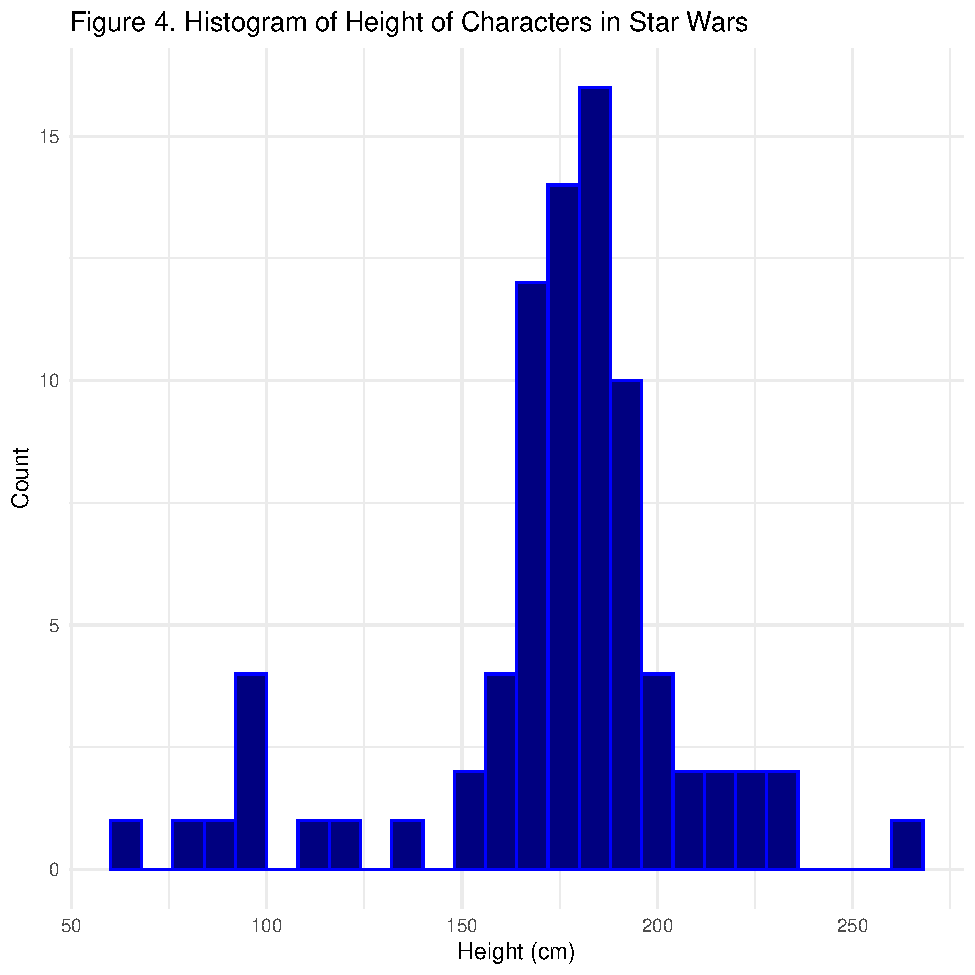
\includegraphics[keepaspectratio]{summarystatisticspdf_files/figure-pdf/unnamed-chunk-21-1.pdf}}

Now, we filter the species to get visual pattern of the height of
different \emph{human} characters in Star Wars.

\begin{Shaded}
\begin{Highlighting}[]
\NormalTok{starwars }\SpecialCharTok{\%\textgreater{}\%}
  \FunctionTok{filter}\NormalTok{(species }\SpecialCharTok{==} \StringTok{"Human"}\NormalTok{) }\SpecialCharTok{\%\textgreater{}\%}
  \FunctionTok{ggplot}\NormalTok{(}\FunctionTok{aes}\NormalTok{(}\AttributeTok{x =}\NormalTok{ height)) }\SpecialCharTok{+}
  \FunctionTok{geom\_histogram}\NormalTok{(}\AttributeTok{binwidth =} \DecValTok{8}\NormalTok{, }\AttributeTok{fill =} \StringTok{"navy"}\NormalTok{, }\AttributeTok{color =} \StringTok{"blue"}\NormalTok{) }\SpecialCharTok{+}
  \FunctionTok{labs}\NormalTok{(}
    \AttributeTok{title =} \StringTok{"Figure 5. Histogram of Height of Human Characters in Star Wars"}\NormalTok{,}
    \AttributeTok{x =} \StringTok{"Height (cm)"}\NormalTok{,}
    \AttributeTok{y =} \StringTok{"Count"}
\NormalTok{  ) }\SpecialCharTok{+}
  \FunctionTok{theme\_minimal}\NormalTok{()}
\end{Highlighting}
\end{Shaded}

\begin{verbatim}
Warning: Removed 5 rows containing non-finite outside the scale range
(`stat_bin()`).
\end{verbatim}

\pandocbounded{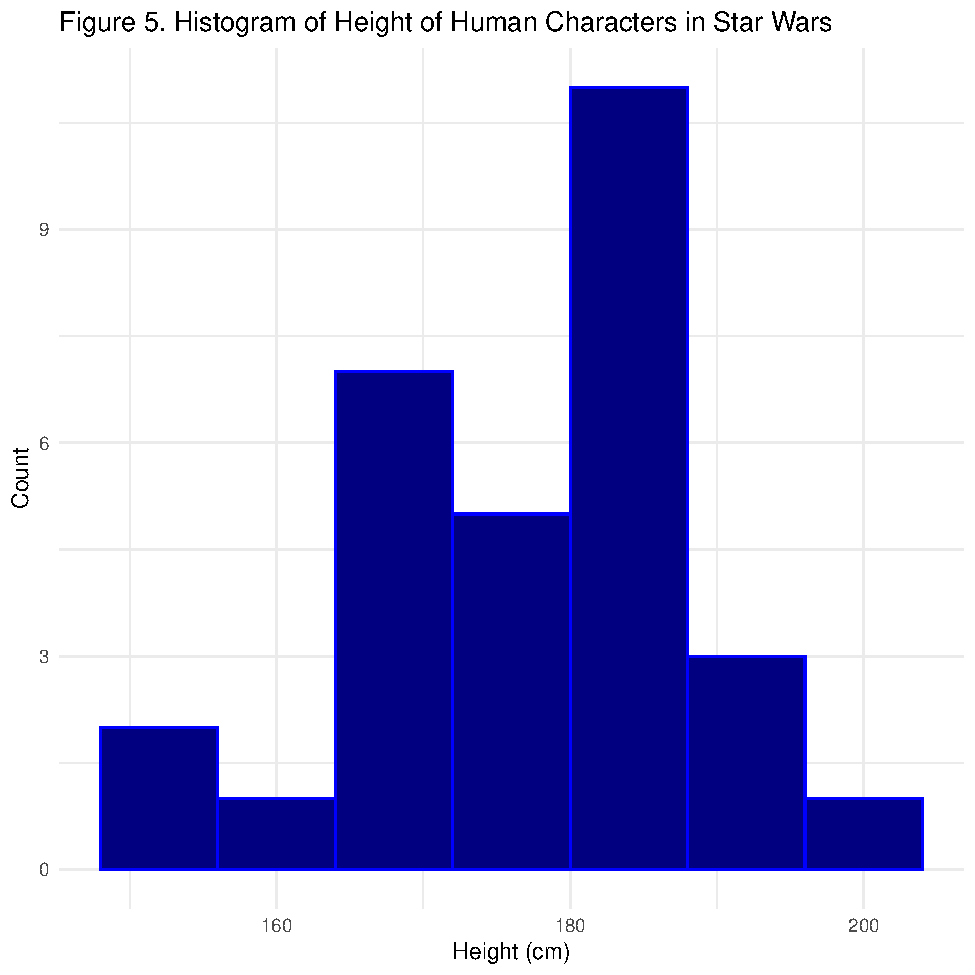
\includegraphics[keepaspectratio]{summarystatisticspdf_files/figure-pdf/unnamed-chunk-22-1.pdf}}

Furthermore, this YouTube video
\href{https://www.youtube.com/watch?v=4vSfbz9YMa0}{Return of the Star
Wars dataset} may be an interesting resource to help you better
understand the dataset.

\newpage

\section{Limitations}\label{limitations}

Summary statistics are essential for providing a quick and accessible
overview of a dataset, but they have several important limitations. In
the book \emph{Naked Statistics}
(\citeproc{ref-wheelan2013naked}{Wheelan, 2013}), the author highlights
key limitations of statistics, warning that statistical measures can be
easily misapplied, misinterpreted, or manipulated to mislead people. He
explains that while statistics help summarize complex data, this
simplification can lead to information loss and oversights, especially
when descriptive statistics are mistaken for complete truth. He
emphasizes that statistics are only as reliable as the data and methods
behind them, and that issues like bias, poor sampling, or careless
analysis can produce misleading or false conclusions.

Let's look at some of the limitations in detail:

\begin{itemize}
\item
  No Causality or Explanation: Summary statistics describe what is
  present in the data but cannot explain why patterns exist or establish
  causal relationships. For example, knowing the average test score does
  not reveal the factors that influenced those scores.
\item
  Limited to the Sample: These statistics only summarize the data
  actually measured and cannot be generalized to a broader population
  without further inferential analysis. They do not account for sampling
  variability or external validity.
\item
  No Predictive Power: Summary statistics cannot be used to make
  predictions about future observations or unmeasured data; they are
  purely descriptive.
\item
  Loss of Detail and Nuance: By condensing complex data into single
  values (like the mean or median), summary statistics can obscure
  important patterns, subgroups, or variability within the data. For
  instance, two datasets with the same mean can have very different
  distributions.
\item
  Potential for Misleading Conclusions: Relying solely on summary
  statistics can mask underlying issues such as data bias, or important
  subgroup differences, leading to incomplete interpretations.
\item
  No Insight into Relationships: Summary statistics typically focus on
  individual variables and do not reveal relationships or associations
  between multiple variables.
\end{itemize}

In summary, while summary statistics are valuable for initial data
exploration, they should be complemented with more detailed analyses and
visualizations to avoid oversimplification and misinterpretation of the
data.

Other sources: (\citeproc{ref-wienclaw2009misuse}{Wienclaw, 2009})

\newpage

\section{Future Direction}\label{future-direction}

The future of summary statistics is changing as data becomes more
complex, computers get faster, and artificial intelligence is used more
often. Some important trends are emerging:

\begin{itemize}
\item
  Integration with Advanced Computational Methods: As data gets bigger
  and more complicated, summary statistics will be used alongside
  advanced computer methods like bootstrapping, simulations, and machine
  learning. These tools help create stronger and more detailed
  summaries, especially when dealing with complex or messy data.
  (\citeproc{ref-oscgarden2023bootstrapping}{Garden, 2023})
\item
  AI-Driven and Automated Summarization: AI and automation are changing
  how we create and use summary statistics. Tools that use artificial
  intelligence can quickly turn large and complex data into useful
  information, making the process faster and easier. In the future,
  these tools will likely give real-time and personalized summaries,
  helping people get the exact information they need.
  (\citeproc{ref-datatas2025future}{Datatas, 2025})
\item
  Enhanced Visualization and Exploratory Data Analysis: As computer
  graphics and interactive tools improve, visualizations will become
  even more important for summary statistics. This will make it easier
  to explore and understand data, spot patterns, and find unusual
  values, going beyond just using tables or simple charts.
  (\citeproc{ref-potter2010visualizing}{Potter et al., 2010})
\item
  Addressing Big Data and Complex Structures: Summary statistics will
  have to change to handle big data, which includes huge amounts of
  information, different kinds of data, and complex patterns. New ways
  of thinking and new tools will be needed to quickly and effectively
  summarize this information.(\citeproc{ref-fan2014challenges}{Fan et
  al., 2014})
\end{itemize}

In summary, summary statistics are becoming more advanced and will be
part of smarter, more interactive analysis tools. As data gets bigger
and more complex, and as technology and teamwork improve, summary
statistics will remain important for understanding information.

\newpage

\section{Conclusion}\label{conclusion}

Summary statistics are a key starting point for any data analysis,
helping us quickly understand and interpret data. In R, these
statistics---like the mean, median, and standard deviation---give a
clear overview of the data and help spot problems or unusual values. R
makes it easy to calculate these numbers for all the data or for
different groups, using built-in functions and packages like dplyr.

As (\citeproc{ref-lane2013descriptive}{Lane, 2013}) explains, using R to
automate summary statistics saves time and helps organize your analysis.
This basic step is important before moving on to more advanced methods.
By mastering summary statistics in R, you can find useful patterns, make
better decisions, and clearly share your results in research or
business.

\newpage

\section{References}\label{references}

\phantomsection\label{refs}
\begin{CSLReferences}{1}{0}
\bibitem[\citeproctext]{ref-datatas2025future}
Datatas. (2025, April 14). \emph{The future of AI-generated data
summarization for large reports}.
\url{https://datatas.com/the-future-of-ai-generated-data-summarization-for-large-reports/}

\bibitem[\citeproctext]{ref-fan2014challenges}
Fan, J., Han, F., \& Liu, H. (2014). Challenges of big data analysis.
\emph{National Science Review}, \emph{1}(2), 293--314.
\url{https://doi.org/10.1093/nsr/nwt032}

\bibitem[\citeproctext]{ref-oscgarden2023bootstrapping}
Garden, O. (2023, November 27). \emph{The 8 most important statistical
ideas: Bootstrapping and simulation-based inference}.
\url{https://osc.garden/blog/bootstrapping-and-simulation-based-inference/}

\bibitem[\citeproctext]{ref-lane2013descriptive}
Lane, D. M. (2013). Descriptive statistics. In \emph{Introduction to
statistics}. Rice University.
\url{https://onlinestatbook.com/2/introduction/descriptive.html}

\bibitem[\citeproctext]{ref-oh2023making}
Oh, D. M., \& Pyrczak, F. (2023). \emph{Making sense of statistics: A
conceptual overview}. Routledge.

\bibitem[\citeproctext]{ref-potter2010visualizing}
Potter, K., Kniss, J., Riesenfeld, R., \& Johnson, C. R. (2010).
Visualizing summary statistics and uncertainty. \emph{Computer Graphics
Forum}, \emph{29}(3), 823--832.
\url{https://www.sci.utah.edu/~kpotter/publications/potter-2010-VSSU.pdf}

\bibitem[\citeproctext]{ref-Schork2021}
Schork, J. (2021). \emph{How to calculate summary statistics for the
columns of a data frame in r (example code)}. YouTube; Statistics Globe.
\url{https://www.youtube.com/watch?v=FMRkUqy1Sjw}

\bibitem[\citeproctext]{ref-dre2024gentle}
Videos, D. E. R. (2024). \emph{Gentle r \#4: Basic summary statistics in
r with r studio {[}video{]}}. YouTube.
\url{https://www.youtube.com/watch?v=8XFmPP93w_Y}

\bibitem[\citeproctext]{ref-walker2023gtsummary}
Walker, L. (2023). \emph{Easy summary tables in r with gtsummary
{[}video{]}}. YouTube. \url{https://www.youtube.com/watch?v=gohF7pp2XCg}

\bibitem[\citeproctext]{ref-wheelan2013naked}
Wheelan, C. (2013). \emph{Naked statistics: Stripping the dread from the
data}. W. W. Norton \& Company.

\bibitem[\citeproctext]{ref-dplyr2023}
Wickham, H., François, R., Henry, L., Müller, K., \& Vaughan, D. (2023).
\emph{Dplyr: A grammar of data manipulation}.
\url{https://dplyr.tidyverse.org/articles/dplyr.html}

\bibitem[\citeproctext]{ref-wienclaw2009misuse}
Wienclaw, R. A. (2009). The misuse of statistics. \emph{The Research
Starters Sociology}, 1--5.

\end{CSLReferences}

\newpage

\section{Affadative}\label{affadative}

I hereby affirm that this submitted paper was authored unaided and
solely by me. Additionally, no other sources than those in the reference
list were used. Parts of this paper, including tables and figures, that
have been taken either verbatim or analogously from other works have in
each case been properly cited with regard to their origin and
authorship. This paper either in parts or in its entirety, be it in the
same or similar form, has not been submitted to any other examination
board and has not been published.

I acknowledge that the university may use plagiarism detection software
to check my thesis. I agree to cooperate with any investigation of
suspected plagiarism and to provide any additional information or
evidence requested by the university.

Checklist:

\begin{itemize}
\tightlist
\item[$\boxtimes$]
  The handout contains 3-5 pages of text.
\item[$\boxtimes$]
  The submission contains the Quarto file of the handout.
\item[$\boxtimes$]
  The submission contains the Quarto file of the presentation.
\item[$\boxtimes$]
  The submission contains the HTML file of the handout.
\item[$\boxtimes$]
  The submission contains the HTML file of the presentation.
\item[$\boxtimes$]
  The submission contains the PDF file of the handout.
\item[$\boxtimes$]
  The submission contains the PDF file of the presentation.
\item[$\boxtimes$]
  The title page of the presentation and the handout contain personal
  details (name, email, matriculation number).
\item[$\boxtimes$]
  The handout contains a abstract.
\item[$\boxtimes$]
  The presentation and the handout contain a bibliography, created using
  BibTeX with APA citation style.
\item[$\boxtimes$]
  Either the handout or the presentation contains R code that proof the
  expertise in coding.
\item[$\boxtimes$]
  The handout includes an introduction to guide the reader and a
  conclusion summarizing the work and discussing potential further
  investigations and readings, respectively.
\item[$\boxtimes$]
  All significant resources used in the report and R code development.
\item[$\boxtimes$]
  The filled out Affidavit.
\item[$\boxtimes$]
  A concise description of the successful use of Git and GitHub, as
  detailed here: \url{https://github.com/hubchev/make_a_pull_request}.
\item[$\boxtimes$]
  The link to the presentation and the handout published on GitHub.
\end{itemize}

Jelin George, 28May2025, Cologne






\end{document}
